% toggles back at the end of this file!
\changemenucolor{gray}{bg}{named}{ese_bg_color} %background of the menukeys
\changemenucolor{gray}{br}{named}{ese_fg_color} %border of the menukeys
\changemenucolor{gray}{txt}{named}{ese_fg_color} %text of the menukeys

\newcommand{\semester}[1]{\minisec{\Large\vspace{.7\baselineskip} #1. Semester\\[.6\baselineskip]}}
\newcommand{\modul}[1]{\vspace{.5\baselineskip}\textbf{\menu[;]{#1\,}}\\[.2\baselineskip]}

\addchap{Modulübersicht}
\addcontentsline{toc}{chapter}{Modulübersicht \hspace*{.15cm} \keys{must read}}

Hier findest du eine kurze Übersicht der Module, die du im Laufe deines Studiums besuchen wirst. Die Reihenfolge ist nicht bindend, es ist lediglich der empfohlene Weg durch das Studium.
Die Symbole \textbf{\menu[;]{I;M;D}} kennzeichnen jeweils die Module für Bachelor Informatik, Bachelor Medieninformatik und Diplom Informatik.

\semester{1}

\modul{I; M; D; Einführung in die Mathematik für Informatiker}
Du kennst dich mit Matrizen aus?
Dann weißt du auch was mit den Begriffen Determinante, Diagonalisierbarkeit, Skalarprodukt und der Lösung eines homogenen linearen Gleichungssystems anzufangen -- wenn nicht, dann lernst du es hier von der Pike auf.
Außerdem wird in der Diskreten Mathematik das Mal und Plus quasi neu definiert und du lernst ein wenig anders zu denken.

\modul{I; M; D; Algorithmen und Datenstrukturen}
Was kommt zuerst?
5 oder 3?
Solche Fragen werden dich in Algorithmen und Datenstrukturen beschäftigen, während du Quicksort, Heapsort und Konsorten kennenlernst.
% Der Wortwitz gefällt mir...
Außerdem wirst du dich in der Gartenarbeit versuchen, indem du AVL- und andere Bäume wachsen lasst.
Dabei wirst du Bekanntschaft mit der Programmiersprache C machen.

\modul{I; M; D; Einführungspraktikum}
Du hast schon immer gerne mit Lego gespielt?
Dann wird dir dieses Praktikum, welches in der vorlesungsfreien Zeit stattfindet, gefallen.
Du darfst dich im Team der Aufgabe stellen, einem selbst konstruierten Roboter in Python beizubringen, wie er sich in einem Labyrinth allein zurechtfindet.
Dabei, und im anschließenden Wettbewerb, kommt der Spaß nicht zu knapp.
Für Diplomstudierende gibt es zusätzlich ein einwöchiges Einzelprojekt, bei dem du zeigen kannst, was du in C oder wahlweise C++ drauf hast. Alternativ kann dieses Strategiespielepraktikum auf das Sommersemester verschoben werden.
In den letzten Jahren war eine künstliche Intelligenz für bekannte Brettspiele gefragt.

\newpage

\modul{I; M; Einführung in die Medieninformatik}
Wie die menschliche Wahrnehmung funktioniert und wie du Software dazu passend ergonomisch gestalten kannst, lernst du in diesem Modul.
Außerdem werden dir verschiedene Eigenschaften der Information und Datenformate anhand der Medien Text, Bild, Audio und Video vorgestellt.
Im Bereich Text und Bild werden die entsprechenden Dokumentenformate des Internets (HTML und SVG) besprochen.
Außerdem erwartet dich ein kurzer Exkurs in die App-Entwicklung.
Ein weiterer Teil des Moduls gibt einen Überblick zur Dokumentenverarbeitung mittels XML-Techniken.
In Übungen und in Form eines Projektes in einer kleinen Gruppe über das Semester hinweg hast du die Möglichkeit, das Erlernte direkt in die Praxis umzusetzen.

\modul{D; Technische Grundlagen und Hardwarepraktikum}
Wenn du schon immer mal wissen wolltest, was die Elektronen im häuslichen Rechner eigentlich so alles durchmachen müssen, bekommst du genau das hier vermittelt.
Anfangs wirst du Transistor-, Dioden- und Operationsverstärkerschaltungen betrachten.
Darauf aufbauend nimmst du Verknüpfungsglieder und komplexe Schaltungen näher unter die Lupe.
Im folgenden Semester kannst du all das hier gelernte dann praktisch anwenden, um selbst ein paar Schaltungen zusammen zu stöpseln.

\modul{D; Rechnerarchitektur}
Hier geht es um die Grundbausteine eines Computers:
Speicher, Bussysteme, Rechen- und Steuerwerk.
Binärcode lesen? Alles Quatsch! In diesem Modul lernst du, wie Maschinensprache wirklich aussieht und bekommst einen kleinen Crash-Kurs in Assembler.
Außerdem schaust du dir das Pipeline-Prinzip an und wirst mit den damit auftretenden Problemen konfrontiert.
Schließlich wird noch diskutiert, mit welchen Methoden du heutige Rechnerarchitekturen beschleunigen und parallele Architekturen nutzen kannst.

\vfill

\begin{figure}[h!]
\centering
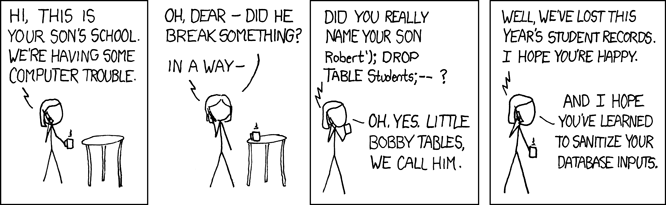
\includegraphics[scale=.5]{img/xkcd/exploits_of_a_mom.png}
\caption*{{\small \textit{Her daughter is named Help I'm trapped in a driver's license factory. (https://xkcd.com/327)}}}
\end{figure}

\semester{2}

\modul{I; M; D; Mathematische Methoden für Informatiker}
Nachdem der Abistoff viel tiefer als vorher sitzt, geht es in den nächsten zwei Semestern in neue Bereiche der Mathematik.
Anfangs wirst du die verschiedenen Typen algebraischer Strukturen (das sind Mengen von beliebigen Symbolen und darauf erklärte Rechenoperationen) untersuchen.
Es folgen Vektoren, Matrizen und mathematische Körper.
Dann kommt ein Sprung vom Diskreten zum Kontinuierlichen.
So langweilig wie in der Schule ist Analysis nämlich gar nicht, die gibt es auch in der Ausführung mit mehreren Veränderlichen.
Das Ganze gipfelt in der Einführung von Differentialgleichungen.
Gegen Schluss wendest du dich erneut den Polynomen zu.
Dabei werden zunächst effiziente Näherungsverfahren behandelt, später folgt noch ein kurzer Ausflug in die Stochastik.

\modul{I; M; D; Programmierung}
Dass Programmiersprachen nicht auf Bäumen wachsen, wusstest du wahrscheinlich schon, doch dass sie strengen mathematischen Regeln folgen, lernst du hier.
Am Beispiel eines Teils der Programmiersprache C wird zunächst die Syntax mit Hilfe von Grammatiken definiert.
Kurz darauf kommst du mit der funktionalen Programmiersprache Haskell in Kontakt und lernst so einen ganz neuen Programmieransatz kennen.
Durch viele hübsche, rekursiv verschachtelte Abbildungen wird dann die Semantik festgelegt, d.h.\ die Wirkung, die so ein Programm auf einer (abstrakten) Rechenmaschine hat.
Außerdem wird hier vermittelt, wie du die Korrektheit eines Programmstückes formal beweist.

\modul{I; M; D; Softwaretechnologie}
Software zu entwickeln ist eine Kunst und gute Software zu schreiben keine einfache Sache, das wirst du spätestens nach diesem Modul erkennen.
Um diese Kunstfertigkeit an den Tag legen zu können, bedarf es einiger Handwerkszeuge, welche du hier mit auf den Weg bekommst.
So werden dir hilfreiche Konzepte am Beispiel von Java und Entwurfsverfahren zusammen mit professioneller Dokumentation nähergebracht.
Damit wird dann der Grundstein für das Projekt im dritten Semester gelegt, bei dem du dir Lorbeeren im Projektmanagement und in der Softwareentwicklung verdienen kannst.


\newpage

\modul{I; D; Informations- und Kodierungstheorie}
Was Informationen eigentlich sind und was sie ausmacht, wird dich hier beschäftigen.
Im Mittelpunkt steht am Anfang, wie du Informationen darstellen und speichern kannst.
Etwas später wird dir erklärt, warum und wie die Informationen mittels Kodierung geschützt werden, damit sie bei dir sicher ankommen, wenn sie unterwegs Störungen und Manipulationen ausgesetzt sind.
Dabei wird dir dein bisher in der Mathematik erworbenes Wissen von Nutzen sein.

\modul{I; Einführung in die Computergraphik}
Was steckt eigentlich hinter der Unreal Engine? Wie funktionieren Shader?
Wieso sehen die Figuren in Computerspielen immer realistischer aus?
Das erfährst du in diesem Modul, zusammen mit dem Aufbau von Grafiksystemen, Farbräumen, Rastergrafiken und deren Anwendungen.
Bestehende Probleme wie Aliasing und Artefakte sind mit von der Partie, sowie ihre algorithmischen Lösungen.
Als Programmiersprache für die Übungsaufgaben wird C++ genutzt.

\modul{M; Grundlagen der Gestaltung}
In dieses Modul lernst du Begriffsdefinitionen sowie allgemeinen Prinzipien der Gestaltung kennen.
Dabei beschränkt sich die Veranstaltung bewusst auf zweidimensionale Bereiche.
Formkategorien, Kontrastbildung und Farblehre bilden die Schwerpunkte.
Die begleitenden Übungen sollen dir einen Einblick in die Materie vermitteln und deine Sensibilität durch handwerkliches Arbeiten wecken.

\modul{M; Medien und Medienströme}
Hier wird dir Wissen zu Medien, deren Kompression und Bearbeitung vermittelt.
Die Anwendung verschiedener Werkzeuge zur Erzeugung von Medien und deren Charakteristika sind ebenfalls Gegenstand dieser Lehrveranstaltung.
So wirst du dich in Form von Übungsaufgaben mit den Grundlagen der Bild-, Audio- und Videobearbeitung auseinandersetzen.

\modul{D; Rechnerarchitektur}
Fortsetzung aus dem 1. Semester.

\modul{D; Technische Grundlagen und Hardwarepraktikum}
Fortsetzung aus dem 1. Semester. Schaltskizzen und physikalische Gesetze -- schön und gut. Aber wie passt das alles zusammen?
Darum soll es in diesem Modul gehen. In einer Reihe von Experimenten wirst du all das gelernte mal praktisch anwenden.
Von analogen über digitale bis hin zu einem eigenen kleinen Computer ist alles mit dabei!

\newpage

\semester{3}

\modul{I; M; D; Mathematische Methoden für Informatiker}
Fortsetzung aus dem 2. Semester.

\modul{I; M; D; Softwaretechnologie-Projekt}
Das Projekt nimmt den größten Teil des dritten Semesters ein.
Hier musst du dein Wissen aus der Lehrveranstaltung \enquote{Softwaretechnologie} in die Tat umsetzen.
In einem fünfköpfigen Team hast du die Aufgabe, eine Anwendung für einen reale Kundschaft oder den Lehrstuhl zu schreiben.
Dabei müsst ihr euch als Team um die Konzeption, Planung, Programmierung und Arbeitsteilung kümmern.
Ihr haltet Rücksprache mit der Kundschaft und/oder den Betreungspersonen und vielleicht müsst ihr noch mal alles ändern.
Abgeschlossen wird das Modul mit der Präsentation des fertigen Produkts.
Am Ende hast du dann einen Eindruck, wie die Arbeit im IT-Bereich aussehen kann.

\modul{I; M; D; Formale Systeme}
Wahr?
Und oder falsch?
Was falsch ist wird, wenn es falsch falsch ist, wahr?
Logisch!
Wenn morgen alle einen Schirm dabei haben, wird es regnen?
Neben der Aussagenlogik vermittelt dir dieses Modul die Grundlagen formaler Sprachen.
Es folgen Gedanken zur maschinellen Berechenbarkeit und zur Automatentheorie.
Turing lässt grüßen.

\modul{I; M; Rechnerarchitektur}
Beschreibung siehe 1. Semester.

\modul{I; Technische Grundlagen und Hardwarepraktikum}
Beschreibung siehe 1. Semester.

\modul{M; Einführung in die Mediengestaltung}
Die Vorlesung vermittelt dir die Grundzüge des multimedialen Gestaltens unter Gesichtspunkten der Entwicklung von einzelnen Richtungen (Film, Internet) mit Bezug auf die gestalterischen Änderungen in den vergangenen Jahrhunderten (Buch).
Außerdem eignest du dir die nützliche Methode der Metaphernbildung und Schwerpunkte im Interfacedesign an.

\newpage

\modul{D; Grundlagen des Nebenfachs}
Je nachdem, welches Nebenfach du wählst, beschäftigst du dich hier mit Themen, die nur im entfernten Sinne mit Informatik zusammenhängen.
Über den Tellerrand schauen und andere Welten kennenlernen ist das Motto.
Hier bietet sich dir eine Gelegenheit Studierende aus anderen Fachrichtungen kennenzulernen.

\modul{D; Betriebssysteme und Sicherheit}
In dieser Lehrveranstaltung nimmst du dienstbare Geister, die zwischen der Hardware und den bunten Anwendungen werkeln, unter die Lupe.
Warum kannst du mit einem Rechner gleichzeitig einen Text schreiben, Code kompilieren, ein Bild bearbeiten und Musik hören?
Wie werden deine Daten in Rechnersystemen geschützt?
Wieso stehen viele hier auf dieses Unix?

\semester{4}

\modul{I; M; D; Datenbanken und Rechnernetze}
Wohin mit deinen 20 Terabyte Nutzdaten? Und wie kommt das Youtube-Video eigentlich von den USA in deinen Browser?
Darum wird es in diesem Modul gehen, das aus zwei verschiedenen Lehrveranstaltungen besteht.
In \textit{Datenbanken} lernst du zuerst Methoden zur effizienten Datenspeicherung kennen.
Danach wird dir die Fähigkeit vermittelt, selbst komplexe relationale Datenbanken zu konzipieren und zu erstellen.
In \textit{Rechnernetze} fängst du mit dem Funktionsprinzip von Modem und Netzwerkkarte an und du erhältst einen kurzen Überblick über moderne Kommunikations- und Vermittlungsprotokolle.
Auch der Sektor Mobilkommunikation und die dabei auftretenden Schwierigkeiten werden kurz beleuchtet.

\modul{I; M; Rechnerarchitektur}
Fortsetzung aus dem 3. Semester.

\modul{I; D; Theoretische Informatik und Logik}
Die Fortsetzung der Formalen Systeme.
So betrachtest du die Korrektheit und Terminierung von Algorithmen und deren notwendigen Aufwand in Form von Zeit und Platzbedarf.
Ein Abstecher in die Prädikatenlogik und Logikprogrammierung rundet das Modul ab.

\modul{I; Technische Grundlagen und Hardwarepraktikum}
Fortsetzung aus dem 3. Semester.

\modul{M; Medienpsychologie und -didaktik}
Mediendidaktik ist die \enquote{Kunst des Lehrens}.
Hier werden dir die Fragen beantwortet:
Was ist Bildung?
Wie verläuft sie?
Wie lässt sie sich vervollkommnen?
Du erfährst etwas über die Entwicklung von Lehrmethoden.
Im parallel stattfindenden Praktikum wendest du das Gelernte beim Entwickeln eines Lernspiels an.

\modul{M; Informations- und Kodierungstheorie}
Beschreibung siehe 2. Semester

\modul{M; Einführung in die Computergraphik}
Beschreibung siehe 2. Semester

\modul{M; Medieninformatik-Projekt}
Das große Highlight der Medieninformatik im Bachelor.
In kleineren Gruppen gilt es ein mobiles Spiel, eine Internet-Seite oder etwas anderes Multimediales zu realisieren.
Abgesehen von der Aufgabenstellung sind eurer Fantasie quasi keine Grenzen gesetzt.
Es geht um harte Arbeit, Teamgeist und den gekonnten Umgang mit Schlafmangel, wenn die Deadline schließlich näher rückt.

\modul{D; Grundlagen des Nebenfachs}
Fortsetzung aus dem 3. Semester.

\modul{D; Allg. Basisqualifikationen}
Englisch ist die einzig relevante Sprache für die Informatik.
Hier wird dir vermittelt, wie du dich fachlich auf Englisch ausdrückt.
Falls du mit deinen Englischkenntnissen bereits zufrieden bist, kannst du alternativ einen anderen Sprachkurs oder eine beliebige Lehrveranstaltung aus dem uniweiten Angebot Studium Generale besuchen.
Zusätzlich zu den zwei verpflichtend zu besuchenden Sprachkursen gehört noch ein Proseminar dazu.
Dort wirst du lernen, \textit{wie} du eine wissenschaftliche Veröffentlichung anfertigst -- indem du selbst eine zu einem Thema deiner Wahl schreibst und präsentierst.

\modul{D; Forschungslinie}
Hier erhältst du einen Überblick über aktuelle Forschungsthemen und bekommst vermittelt, wie du forschungsorientiert arbeitest.
Dieses Modul hilft dir, später die richtige Vertiefung zu wählen. Der Besuch dieser Veranstaltung ist auch für Bachelor- und Masterstudierende interessant, vertiefen müssen sie sich schließlich ebenfalls.

\begin{figure}[b!]
\centering
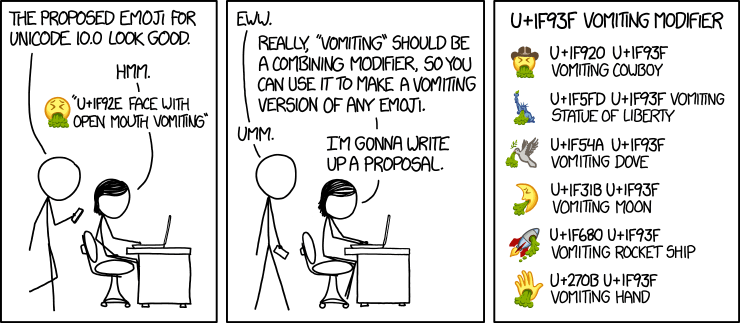
\includegraphics[scale=.4]{img/xkcd/vomiting_emoji.png}
\caption*{{\small \textit{My favorite might be U+1F609 U+1F93F WINKING FACE VOMITING\@. (https://xkcd.com/1813)}}}
\end{figure}

\semester{5}

\modul{I; M; Vertiefung in der Informatik/Medieninformatik}
Hier kannst du aus einem Angebotskatalog geeignete Veranstaltungen wählen, um deinen wissenschaftlichen Horizont zu erweitern.
Die Möglichkeiten beinhalten Vorlesungen, Übungen, Praktika, Exkursionen, Seminare und mehr.

\modul{I; M; Betriebssysteme und Sicherheit}
Beschreibung siehe 3. Semester.

\modul{I; D; Intelligente Systeme}
In diesem Modul geht es um künstliche Intelligenz.
Hier erlernst du Problemlösung, Wissensrepräsentation, Planung und Sprachverarbeitung.
Warum konnte IBM's Watson in \textit{Jeopardy!} gegen die besten menschlichen Spielenden gewinnen?
Woher weiß ein Spamfilter, was Spam ist und was nicht?
Die Antworten darauf, lernst du mit den dafür verwendeten Lernalgorithmen kennen.

\modul{I; D; Systemorientierte Informatik/Hardware Software Codesign}
Dieses Modul behandelt Schnittstellen zwischen Rechnern und industriellen Anlagen.
Zunächst abstrahierst du, was allen vorkommenden Systemen gemein ist, und es werden Begriffe wie \enquote{System}, \enquote{Signal} und \enquote{Regelkreis} formalisiert, mit denen es sich einfacher rechnerisch arbeiten lässt.
Du wirst fit gemacht für die Analyse und Voraussage von Übertragungsverhalten und Reaktionen, die ein solches System bei einer bestimmten Eingabe zeigen wird.
Aspekte der Audio- und Videotechnik wie Digitalisierung und Filterung kommen ebenfalls nicht zu kurz.

\modul{M; Web- und Multimedia Engineering}
Wie kannst du das Web mit heutiger Technik multimedial und interaktiv gestalten? Warum ist HTML5 so toll?
Wie nutzt du professionelle Entwicklungswerkzeuge und geeignete Sprachen, um deine Vorstellung in das Ergebnis zu projizieren?
Dieses Modul hilft geeignete Methoden zu erlernen und Erfahrung bei der Anwendung zu sammeln.

\modul{M; Medieninformatik-Projekt}
Fortsetzung aus dem 4. Semester.

\modul{D; Vertiefung im Nebenfach}
Nachdem du dir die Grundlagen deines gewählten Nebenfachs angeeignet hast, wird es nun ernst und du steigst tiefer in die Materie ein.

\modul{D; Basismodul 1, 2 und 3}
Hier wählst du unter sieben verschiedenen Themenkomplexen drei aus und beschäftigst dich mit ihnen.
Zur Wahl stehen Angewandte Informatik, Künstliche Intelligenz, Software- und Web-Engineering, Systemarchitektur, Technische Informatik, Theoretische Informatik sowie Graphische Datenverarbeitung.
Innerhalb dieser Richtungen stehen dir passende Veranstaltungen zur Auswahl.

\semester{6}

\modul{I; M; Spezialisierung in der Informatik/Medieninformatik}
Weitere Vertiefung nach gleichem Muster wie im fünften Semester in Vorbereitung auf die Bachelorarbeit.

\modul{I; M; Überfachliche Qualifikation}
In dieser Art Nebenfach orientierst du dich fächerübergreifend an Themen deines Interesses, um die fachspezifische Kompetenz zu entwickeln.
Außerdem ist dieses Modul ein weiterer guter Zeitpunkt, um eine neue Sprache zu lernen. Japanisch? Arabisch? Russisch? Oder doch nochmal Englisch?
Auch hier können Veranstaltungen aus einem Katalog gewählt werden.

\newpage

\modul{I; M; Bachelorarbeit und Kolloquium}
Als krönenden Abschluss fertigst du deine Bachelorarbeit zu einem Thema deiner Wahl an und verteidigst sie in einem Vortrag.
Glückwunsch! Du bist nun offiziell \textit{Bachelor of Science}! Wie wäre es mit einem Master-Studium im Anschluss?

\modul{D; Vertiefung im Nebenfach}
Fortsetzung aus dem 5. Semester.

\modul{D; Basismodul 1, 2 und 3}
Fortsetzung aus dem 5. Semester.

\semester{7.\ bis 10}

Im Studiengang Diplom Informatik hast du nach den ersten sechs Semestern noch vier weitere vor dir. Gleichzeitig werden die meisten Bachelorstudierenden eine Masterstudiengang wählen.
Während des siebten Semesters wirst du ein Berufspraktikum absolvieren, hier bietet sich dir außerdem eine ideale Gelegenheit für einen Auslandsaufenthalt.
Im achten und neunten wirst du dann Module auswählen, die dich interessieren, tiefer in die Abgründe deines gewählten Themas hinabsteigen, dir weitere Kompetenzen nach dem selben Prinzip wie in \enquote{Allgemeine Basisqualifikationen} aneignen, einen \enquote{Großen Beleg} (vergleichbar mit der Bachelorarbeit) schreiben und weitere Arbeiten anfertigen.
Und im zehnten, letzten Semester schreibst du schlussendlich deine Diplomarbeit und das war es dann schon!
So schnell kann es gehen.

\begin{figure}[b!]
\centering
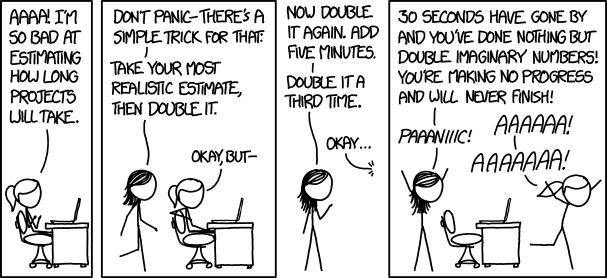
\includegraphics[width=.73\textwidth]{img/xkcd/estimating_time.png}
\caption*{\centering {\small \textit{Corollary to Hofstadter's Law: Every minute you spend thinking about Hofstadter's Law is a minute you're NOT WORKING AND WILL NEVER FINISH\@! PAAAAAANIIIIIIC\@! (https://xkcd.com/1658/)}}}
\end{figure}

\changemenucolor{gray}{bg}{named}{ese_fg_color} %background of the menukeys
\changemenucolor{gray}{br}{named}{ese_bg_color} %border of the menukeys
\changemenucolor{gray}{txt}{named}{ese_bg_color} %text of the menukeys
